%=======================================================================
%  LLM-Driven End-to-End PCB Generation for KiCad  (PCBSchemaGen)
%  1-hour technical review  |  Dushyant Singh
%  Compile:  pdflatex -interaction=nonstopmode pcbschemagen_talk.tex  (x2)
%  Images:   drop files into ./figures/ with the names shown in the
%            dashed placeholder boxes; they are picked up automatically.
%=======================================================================
\documentclass[aspectratio=169,10pt]{beamer}

\usepackage[T1]{fontenc}
\usepackage[utf8]{inputenc}
\usepackage{helvet}
\usepackage{courier}
\usepackage{graphicx}
\usepackage{booktabs}
\usepackage{array}
\usepackage{listings}
\usepackage{tikz}
\usetikzlibrary{positioning,shapes.geometric,shapes.misc,arrows,calc,fit,backgrounds,decorations.pathreplacing,chains}

%-----------------------------------------------------------------------
%  Theme : minimal custom (ST-inspired palette)
%-----------------------------------------------------------------------
\usetheme{default}
\usecolortheme{default}
\setbeamertemplate{navigation symbols}{}
\renewcommand{\familydefault}{\sfdefault}

\definecolor{stblue}{HTML}{03234B}   % ST deep blue
\definecolor{stcyan}{HTML}{3CB4E6}   % ST light blue
\definecolor{stgrey}{HTML}{5A6672}
\definecolor{stlight}{HTML}{E8EEF4}
\definecolor{stgreen}{HTML}{1E8449}
\definecolor{stamber}{HTML}{C87F0A}
\definecolor{stred}{HTML}{A93226}

\setbeamercolor{structure}{fg=stblue}
\setbeamercolor{frametitle}{fg=white,bg=stblue}
\setbeamercolor{title}{fg=stblue}
\setbeamercolor{itemize item}{fg=stcyan}
\setbeamercolor{itemize subitem}{fg=stgrey}
\setbeamercolor{block title}{fg=white,bg=stblue}
\setbeamercolor{block body}{bg=stlight}
\setbeamercolor{alerted text}{fg=stred}
\setbeamerfont{frametitle}{size=\large,series=\bfseries}
\setbeamertemplate{itemize item}{\raisebox{0.15ex}{\tiny$\blacksquare$}}
\setbeamertemplate{itemize subitem}{\raisebox{0.15ex}{\tiny$\square$}}
\setbeamertemplate{blocks}[rounded][shadow=false]

% frame title with a thin cyan rule underneath
\setbeamertemplate{frametitle}{%
  \nointerlineskip
  \begin{beamercolorbox}[wd=\paperwidth,ht=2.6ex,dp=1.2ex,leftskip=0.3cm,rightskip=0.3cm]{frametitle}
    \usebeamerfont{frametitle}\insertframetitle
  \end{beamercolorbox}%
  \nointerlineskip
  \begin{beamercolorbox}[wd=\paperwidth,ht=0.6mm,dp=0mm]{}\hbox{}\end{beamercolorbox}%
  \vskip-0.6mm\hbox{\color{stcyan}\rule{\paperwidth}{0.6mm}}
}

% footline : short title | section | slide number
\setbeamertemplate{footline}{%
  \hbox{\begin{beamercolorbox}[wd=\paperwidth,ht=2ex,dp=0.8ex,leftskip=0.3cm,rightskip=0.3cm]{}%
    \tiny\color{stgrey}PCBSchemaGen \textbullet\ LLM-Driven End-to-End PCB Generation for KiCad
    \hfill \insertsectionhead \hfill \insertframenumber/\inserttotalframenumber
  \end{beamercolorbox}}%
}

%-----------------------------------------------------------------------
%  Helpers
%-----------------------------------------------------------------------
\newcommand{\ok}{{\color{stgreen}\textbf{\checkmark}}}
\newcommand{\gap}{{\color{stamber}\textbf{!}}}
\newcommand{\no}{{\color{stred}\textbf{$\times$}}}
\newcommand{\code}[1]{{\ttfamily\small #1}}

\lstdefinestyle{sh}{
  basicstyle=\ttfamily\scriptsize,
  backgroundcolor=\color{stlight},
  keywordstyle=\color{stblue}\bfseries,
  commentstyle=\color{stgrey}\itshape,
  stringstyle=\color{stgreen},
  breaklines=true, breakatwhitespace=false,
  frame=leftline, framerule=1.2pt, rulecolor=\color{stcyan},
  xleftmargin=6pt, framexleftmargin=6pt, framexrightmargin=3pt,
  framextopmargin=3pt, framexbottommargin=3pt,
  showstringspaces=false, columns=fullflexible,
  literate={\$}{{\textcolor{stcyan}{\$}}}1
}
\lstset{style=sh}

% TikZ node styles for the flowcharts
\tikzset{
  stg/.style   ={rectangle, rounded corners=2pt, draw=stblue, very thick,
                 fill=white, text=stblue, align=center, font=\scriptsize\bfseries,
                 minimum height=8mm, minimum width=17mm, inner sep=3pt},
  stgf/.style  ={stg, fill=stblue, text=white},
  stgc/.style  ={stg, fill=stcyan!25},
  art/.style   ={rectangle, draw=stgrey, thick, dashed, fill=stlight,
                 align=center, font=\tiny\ttfamily, text=stgrey,
                 minimum height=6mm, inner sep=3pt},
  chk/.style   ={diamond, aspect=1.9, draw=stamber, very thick, fill=stamber!12,
                 align=center, font=\scriptsize\bfseries, text=stblue, inner sep=1pt},
  ext/.style   ={rectangle, draw=stgreen, very thick, fill=stgreen!10,
                 align=center, font=\scriptsize\bfseries, text=stgreen!60!black,
                 minimum height=8mm, inner sep=3pt},
  fl/.style    ={-latex, very thick, draw=stblue},
  flb/.style   ={-latex, very thick, draw=stamber, dashed},
  lbl/.style   ={font=\tiny\itshape, text=stgrey, inner sep=1.5pt}
}

%-----------------------------------------------------------------------
\title{\textbf{LLM-Driven End-to-End PCB Generation for KiCad}}
\subtitle{From a natural-language prompt to an ERC-clean schematic and a routed board}
\author{Dushyant Singh\\[2pt]{\small President, Semiconductor Chip Design Club}}
\institute{\small SRM Institute of Science and Technology\\[2pt]
           \scriptsize Mentor: Saurabh Rawat, STMicroelectronics}
\date{\small\today}

%=======================================================================
\begin{document}

{\setbeamertemplate{footline}{}
\begin{frame}[plain]
  \vspace{2mm}
  \begin{center}
  
\begin{tikzpicture}
    \node[fill=stblue,text=white,rounded corners=4pt,inner sep=8pt,align=center,minimum width=0.88\textwidth]
    {\Large\textbf{LLM-Driven End-to-End PCB Generation for KiCad}\\[4pt]
     \color{stcyan}\normalsize PCBSchemaGen};
  \end{tikzpicture}
  \end{center}
  \vspace{1mm}
  \begin{center}
  {\small Natural-language prompt $\rightarrow$ ERC-validated SKiDL netlist $\rightarrow$ native KiCad 9 schematic $\rightarrow$ DRC-checked routed PCB}\\[6mm]
  {\normalsize\textbf{Dushyant Singh}}\\[2pt]
  {\footnotesize President, Semiconductor Chip Design Club \textbullet\ SRM IST}\\[4mm]
  {\footnotesize Mentor: \textbf{Saurabh Rawat}, STMicroelectronics}\\[6mm]
  {\scriptsize\color{stgrey}Technical Review \textbullet\ \today}
  \end{center}
\end{frame}}

%-----------------------------------------------------------------------
\begin{frame}{Agenda}
\vspace{1mm}
\begin{center}
\begin{tabular}{@{}p{0.10\textwidth} p{0.60\textwidth} r@{}}
\toprule
\textbf{Part} & \textbf{Topic} & \textbf{Time} \\
\midrule
\textbf{1} & What the project does --- flow, architecture, and the outputs generated (schematic + layout) & 15 min \\[3pt]
\textbf{2} & How to replicate the work --- environment, dependencies, SKiDL, KiCad, LLM APIs & 15 min \\[3pt]
\textbf{3} & Next tasks --- open gaps, roadmap, and the north-star benchmark & 15 min \\[3pt]
\textbf{4} & \textit{Questions \& discussion} & 15 min \\
\bottomrule
\end{tabular}
\end{center}
\vspace{3mm}
\begin{center}
\footnotesize\color{stgrey}
Total: 60 minutes. Backup material in the appendix for detailed questions.
\end{center}
\end{frame}

%=======================================================================
\section{Part 1 --- What the project does}
%=======================================================================
{\setbeamercolor{background canvas}{bg=stblue}
\begin{frame}[plain]
\vfill
\begin{center}
{\color{stcyan}\Large\textbf{Part 1}}\\[6pt]
{\color{white}\LARGE\textbf{What the project does}}\\[10pt]
{\color{white}\small The flow, the architecture, and the outputs generated}\\[4pt]
{\color{stcyan}\footnotesize 15 minutes}
\end{center}
\vfill
\end{frame}}

%-----------------------------------------------------------------------
\begin{frame}{The problem}
\vspace{1mm}
\begin{columns}[T]
\begin{column}{0.52\textwidth}
\textbf{Today's hardware flow is human-serial}
\begin{itemize}\small
  \item Read datasheet $\rightarrow$ pick parts $\rightarrow$ draw schematic $\rightarrow$ place $\rightarrow$ route $\rightarrow$ check.
  \item Every stage is manual, and every stage is where a silent error enters.
  \item A decoupling cap on the wrong rail, a swapped SPI pin --- none of it is caught until the board is fabricated.
\end{itemize}
\vspace{2mm}
\textbf{Meanwhile, in digital design}
\begin{itemize}\small
  \item RTL $\rightarrow$ GDSII is automated end-to-end and \emph{verified at every handoff}.
  \item PCB design has no equivalent closed loop.
\end{itemize}
\end{column}
\begin{column}{0.46\textwidth}
\begin{block}{The question this project answers}
\small
Can a language model be placed at the \emph{front} of a hardware flow --- as the \textbf{intent} stage --- while deterministic, authoritative tools own every stage after it?
\end{block}
\vspace{2mm}
\begin{block}{Design principle}
\small
The LLM proposes. \textbf{KiCad, SKiDL and the DRC engine dispose.}\\[3pt]
No LLM output ever reaches a file without passing a machine check.
\end{block}
\end{column}
\end{columns}
\end{frame}

%-----------------------------------------------------------------------
\begin{frame}{What PCBSchemaGen is}
\vspace{2mm}
\begin{center}
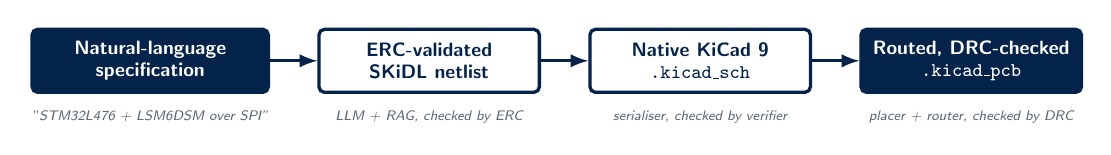
\begin{tikzpicture}[node distance=6mm]
  \node[stgf,minimum width=30mm] (a) {Natural-language\\specification};
  \node[stg,right=of a,minimum width=28mm] (b) {ERC-validated\\SKiDL netlist};
  \node[stg,right=of b,minimum width=28mm] (c) {Native KiCad 9\\\texttt{.kicad\_sch}};
  \node[stgf,right=of c,minimum width=28mm] (d) {Routed, DRC-checked\\\texttt{.kicad\_pcb}};
  \draw[fl] (a)--(b); \draw[fl] (b)--(c); \draw[fl] (c)--(d);
  \node[lbl,below=1.5mm of a] {"STM32L476 + LSM6DSM over SPI"};
  \node[lbl,below=1.5mm of b] {LLM + RAG, checked by ERC};
  \node[lbl,below=1.5mm of c] {serialiser, checked by verifier};
  \node[lbl,below=1.5mm of d] {placer + router, checked by DRC};
\end{tikzpicture}
\end{center}
\vspace{3mm}
\begin{columns}[T]
\begin{column}{0.48\textwidth}
\textbf{Scope}
\begin{itemize}\small
  \item Target vendor: \textbf{STMicroelectronics} parts
  \item Target tool: \textbf{KiCad 9} (native file formats, no round-trip through third-party formats)
  \item Fully headless --- no GUI step anywhere in the flow
\end{itemize}
\end{column}
\begin{column}{0.48\textwidth}
\textbf{Benchmark circuit}
\begin{itemize}\small
  \item \textbf{STM32L476JGYxP} (WLCSP-72) $\leftrightarrow$ \textbf{LSM6DSM} IMU (LGA-14), SPI
  \item 22 components \textbullet\ 68 nets \textbullet\ 126 pads
  \item 7 independent supply rails
\end{itemize}
\end{column}
\end{columns}
\end{frame}

%-----------------------------------------------------------------------
\begin{frame}{End-to-end flow --- the six stages}
\vspace{1mm}
\begin{center}
\resizebox{\textwidth}{!}{%
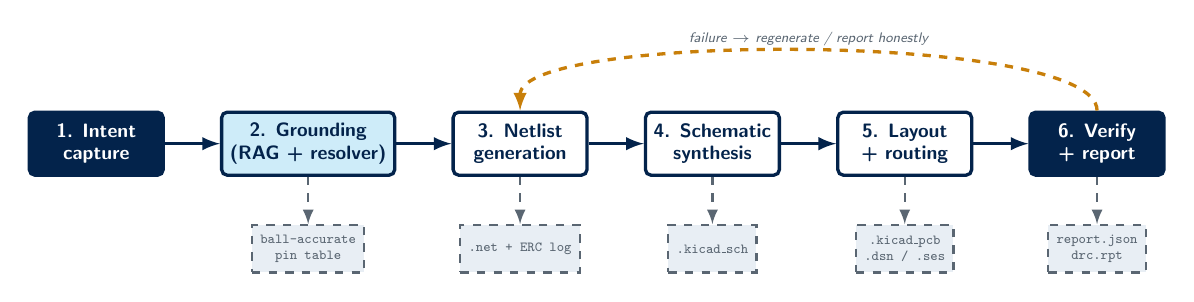
\begin{tikzpicture}[node distance=8mm and 7mm]
  \node[stgf] (s1) {1. Intent\\capture};
  \node[stgc,right=of s1] (s2) {2. Grounding\\(RAG + resolver)};
  \node[stg,right=of s2]  (s3) {3. Netlist\\generation};
  \node[stg,right=of s3]  (s4) {4. Schematic\\synthesis};
  \node[stg,right=of s4]  (s5) {5. Layout\\+ routing};
  \node[stgf,right=of s5] (s6) {6. Verify\\+ report};

  \draw[fl] (s1)--(s2); \draw[fl] (s2)--(s3); \draw[fl] (s3)--(s4);
  \draw[fl] (s4)--(s5); \draw[fl] (s5)--(s6);

  \node[art,below=6mm of s2] (a2) {ball-accurate\\pin table};
  \node[art,below=6mm of s3] (a3) {\texttt{.net} + ERC log};
  \node[art,below=6mm of s4] (a4) {\texttt{.kicad\_sch}};
  \node[art,below=6mm of s5] (a5) {\texttt{.kicad\_pcb}\\\texttt{.dsn / .ses}};
  \node[art,below=6mm of s6] (a6) {\texttt{report.json}\\\texttt{drc.rpt}};
  \draw[-latex,thick,stgrey,dashed] (s2)--(a2);
  \draw[-latex,thick,stgrey,dashed] (s3)--(a3);
  \draw[-latex,thick,stgrey,dashed] (s4)--(a4);
  \draw[-latex,thick,stgrey,dashed] (s5)--(a5);
  \draw[-latex,thick,stgrey,dashed] (s6)--(a6);

  \draw[flb] (s6.north) .. controls +(0,10mm) and +(0,10mm) .. (s3.north)
        node[lbl,midway,above] {failure $\rightarrow$ regenerate / report honestly};
\end{tikzpicture}}
\end{center}
\vspace{2mm}
\begin{center}\footnotesize
Every arrow crosses a \textbf{verification gate}. A stage may only hand forward what the next stage's authoritative tool has accepted.
\end{center}
\end{frame}

%-----------------------------------------------------------------------
\begin{frame}{Phase 1 --- schematic generation (detailed flow)}
\vspace{-1mm}
\begin{center}
\resizebox{\textwidth}{!}{%
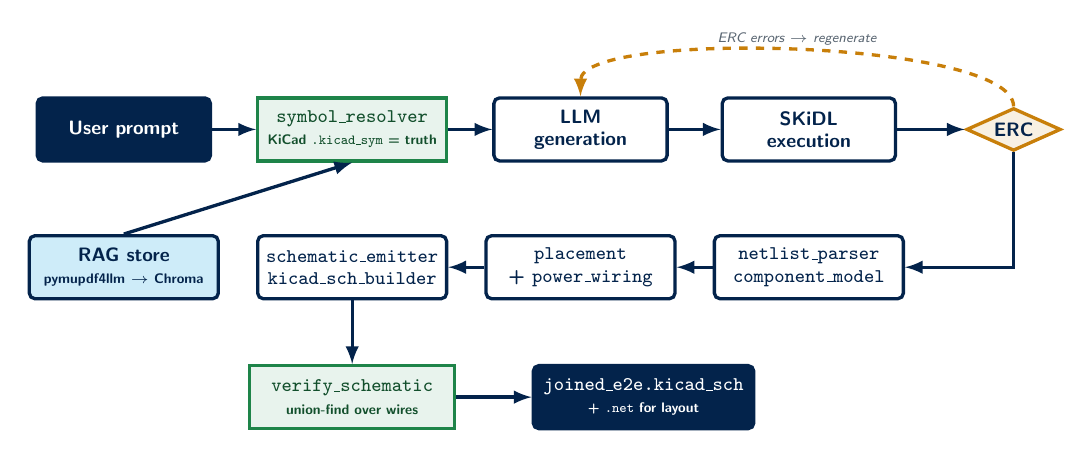
\begin{tikzpicture}[x=1cm,y=1cm]
  % --- row 1 : intent -> generation -> ERC
  \node[stgf,minimum width=22mm]           (p)     at (0,0)      {User prompt};
  \node[ext,minimum width=24mm]            (res)   at (2.9,0)    {\texttt{symbol\_resolver}\\{\tiny KiCad \texttt{.kicad\_sym} = truth}};
  \node[stg,minimum width=22mm]            (llm)   at (5.8,0)    {LLM\\generation};
  \node[stg,minimum width=22mm]            (skidl) at (8.7,0)    {SKiDL\\execution};
  \node[chk,minimum width=12mm]            (erc)   at (11.3,0)   {ERC};
  % --- grounding
  \node[stgc,minimum width=24mm]           (rag)   at (0,-1.75)  {RAG store\\{\tiny pymupdf4llm $\rightarrow$ Chroma}};
  % --- row 2 : netlist -> geometry -> file  (right to left)
  \node[stg,minimum width=24mm]            (np)    at (8.7,-1.75) {\texttt{netlist\_parser}\\\texttt{component\_model}};
  \node[stg,minimum width=24mm]            (pl)    at (5.8,-1.75) {\texttt{placement}\\+ \texttt{power\_wiring}};
  \node[stg,minimum width=24mm]            (em)    at (2.9,-1.75) {\texttt{schematic\_emitter}\\\texttt{kicad\_sch\_builder}};
  % --- row 3 : verify -> deliver
  \node[ext,minimum width=26mm]            (vf)    at (2.9,-3.4)  {\texttt{verify\_schematic}\\{\tiny union-find over wires}};
  \node[stgf,minimum width=28mm]           (out)   at (6.6,-3.4)  {\texttt{joined\_e2e.kicad\_sch}\\{\tiny + \texttt{.net} for layout}};

  \draw[fl] (p)--(res);  \draw[fl] (res)--(llm);
  \draw[fl] (llm)--(skidl); \draw[fl] (skidl)--(erc);
  \draw[fl] (rag.north) -- (res.south);
  \draw[fl] (erc) |- (np);
  \draw[fl] (np)--(pl); \draw[fl] (pl)--(em);
  \draw[fl] (em)--(vf); \draw[fl] (vf)--(out);
  \draw[flb] (erc.north) .. controls +(0,0.85) and +(0,0.85) .. (llm.north)
        node[lbl,midway,above] {ERC errors $\rightarrow$ regenerate};
\end{tikzpicture}}
\end{center}
\vspace{0.5mm}
\begin{center}\scriptsize
\textbf{Two correctness problems, kept strictly separate:} \emph{netlist correctness} is the LLM's job (ERC judges it); \emph{schematic-file correctness} is the serialiser's job (the verifier judges it).
\end{center}
\end{frame}

%-----------------------------------------------------------------------
\begin{frame}{Grounding: why the LLM never invents a pin}
\vspace{1mm}
\begin{columns}[T]
\begin{column}{0.55\textwidth}
\textbf{The failure we designed out}\\[2pt]
\small A model asked for "STM32L476 SPI to an IMU" will happily emit \code{U1['PA5']} --- a name that does not exist on a WLCSP-72 package, where pins are \emph{ball designators} (\code{A1}, \code{H8}, \code{G7}\ldots).
\vspace{3mm}

\textbf{The fix: authoritative pin injection}
\begin{itemize}\small
  \item \code{kicad\_symbol\_parser.py} reads KiCad's own \code{.kicad\_sym} files.
  \item \code{symbol\_resolver.py} produces the exact, ball-accurate pin list for the requested part.
  \item That list is injected into the prompt, with a hard instruction: \emph{use only these strings; never invent, never index numerically}.
\end{itemize}
\end{column}
\begin{column}{0.43\textwidth}
\begin{block}{Authoritative sources own truth}
\small
\begin{tabular}{@{}ll@{}}
\textbf{KiCad} & owns symbols \& footprints\\
\textbf{ST} & owns design intent\\
\textbf{Resolver} & owns pin data\\
\textbf{Fab} & owns DFM floors\\
\end{tabular}
\end{block}
\vspace{1mm}
\begin{block}{RAG v2}
\small
\code{pymupdf4llm} for layout-aware markdown extraction.\\[3pt]
{\footnotesize Plain PyMuPDF mangled the ball-assignment tables into mojibake --- exactly the data the model most needs.}
\end{block}
\end{column}
\end{columns}
\end{frame}

%-----------------------------------------------------------------------
\begin{frame}{ST-style power auto-wiring}
\vspace{1mm}
\begin{columns}[T]
\begin{column}{0.50\textwidth}
\small
Derived by analysing a real ST reference schematic (\textbf{STEVAL-PLC1MIC1}) and encoding its drawing convention.
\vspace{2mm}

\textbf{The atomic ST unit}\\
supply symbol $\rightarrow$ wire $\rightarrow$ junction dot $\rightarrow$ IC pin,\\
decoupling cap tapped at the junction,\\
GND symbol directly beneath.
\vspace{2mm}

\textbf{Exact geometry (all on the 1.27\,mm grid)}
\begin{center}\footnotesize
\begin{tabular}{@{}lr@{}}
\toprule
pin $\rightarrow$ junction & 6.35 mm\\
pin $\rightarrow$ supply symbol & 12.70 mm\\
cap offset & 7.62 mm\\
\bottomrule
\end{tabular}
\end{center}
\end{column}
\begin{column}{0.48\textwidth}
\begin{block}{The routability rule}
\small
Wire a rail \textbf{if} its stacks fit the free space between the neighbouring rails' pins \textbf{and} cross no other pin.\\[3pt]
Otherwise: label it, and place its caps in a dedicated supply region.
\end{block}
\vspace{2mm}
\textbf{Result on the benchmark (7 rails)}
\begin{itemize}\small
  \item \textbf{5 wired A-rails:} VREF\_PLUS, VBAT, VDDA, VDDIO2, VDDUSB
  \item \textbf{2 labelled B-rails:} VDD\_3V3 (3 pins, 8 caps), VDD12 (2 pins)
  \item \ok\ 0 ERC errors, 0 warnings
\end{itemize}
\end{column}
\end{columns}
\end{frame}

%-----------------------------------------------------------------------
\begin{frame}{Verification: two independent judges}
\vspace{1mm}
\begin{center}
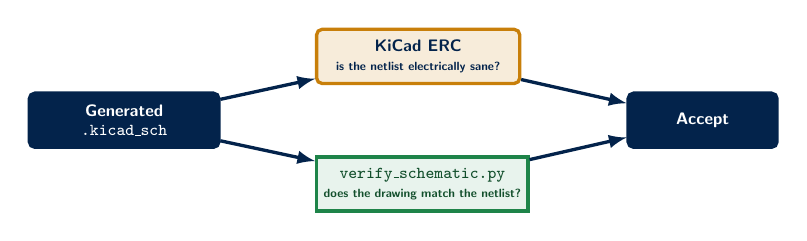
\begin{tikzpicture}[node distance=4mm and 13mm, scale=0.86, transform shape]
  \node[stgf,minimum width=28mm] (sch) {Generated\\\texttt{.kicad\_sch}};
  \node[stg,fill=stamber!15,draw=stamber,above right=1mm and 14mm of sch,minimum width=30mm] (erc)
    {KiCad ERC\\{\tiny is the netlist electrically sane?}};
  \node[ext,below right=1mm and 14mm of sch,minimum width=30mm] (vfy)
    {\texttt{verify\_schematic.py}\\{\tiny does the drawing match the netlist?}};
  \node[stgf,right=14mm of sch,xshift=46mm,minimum width=22mm] (acc) {Accept};
  \draw[fl] (sch) -- (erc); \draw[fl] (sch) -- (vfy);
  \draw[fl] (erc) -- (acc); \draw[fl] (vfy) -- (acc);
\end{tikzpicture}
\end{center}
\vspace{1mm}
\begin{columns}[T]
\begin{column}{0.49\textwidth}
\begin{block}{Two silent faults the verifier caught}
\small
\begin{enumerate}
  \item \textbf{NRST and BOOT0 shorted to VREF\_PLUS} --- an edge-routing bug routed a LEFT-edge rail \emph{along} the pin column. ERC saw nothing.
  \item \textbf{GPIO PC8 touching a B-rail} --- caught only because an \emph{expected} floating-pin error went \emph{missing} from the ERC report.
\end{enumerate}
\end{block}
\end{column}
\begin{column}{0.49\textwidth}
\begin{block}{The principle worth remembering}
\small
\textbf{A disappearing ERC error is worse news than a new one.}\\[4pt]
A new error means something broke loudly. A vanished one means two nets silently merged --- and the check that would have complained is now satisfied by the short itself.
\end{block}
\end{column}
\end{columns}
\end{frame}

%-----------------------------------------------------------------------
\begin{frame}{Output 1 --- the generated schematic}
\vspace{1mm}
\begin{columns}[T]
\begin{column}{0.50\textwidth}
\textbf{What the pipeline produced}
\begin{itemize}\small
  \item A native KiCad 9 \code{.kicad\_sch} --- opened directly in Eeschema, not imported or converted
  \item \textbf{22 components}, \textbf{68 nets}, \textbf{126 pads}
  \item Footprints resolved from KiCad's own libraries, not guessed by the model
  \item Power rails drawn in ST's own convention, on ST's grid
  \item A matching \code{.net} file, which is what Phase 2 consumes
\end{itemize}
\end{column}
\begin{column}{0.47\textwidth}
\begin{block}{Verification status}
\small
\begin{tabular}{@{}l l@{}}
KiCad ERC & \ok\ 0 errors, 0 warnings\\
Independent verifier & \ok\ clean\\
Floating pins & \ok\ all accounted for\\
Duplicate drivers & \ok\ none\\
\end{tabular}
\end{block}
\vspace{1mm}
\begin{block}{The claim this supports}
\small
Not "an LLM drew a schematic." Rather: \textbf{an LLM proposed a netlist, and every downstream artifact was produced and checked by tools that can refuse it.}
\end{block}
\end{column}
\end{columns}
\end{frame}

%-----------------------------------------------------------------------
\begin{frame}{Output 1 --- what the generator decided, rail by rail}
\vspace{1mm}
\begin{center}\small
\begin{tabular}{@{}l c c l l@{}}
\toprule
\textbf{Rail} & \textbf{Pins} & \textbf{Caps} & \textbf{Decision} & \textbf{Why}\\
\midrule
VREF\_PLUS & 1 & 1 & wired A-rail & stacks fit the free space\\
VBAT       & 1 & 1 & wired A-rail & stacks fit the free space\\
VDDA       & 1 & 2 & wired A-rail & stacks fit the free space\\
VDDIO2     & 1 & 1 & wired A-rail & stacks fit the free space\\
VDDUSB     & 1 & 1 & wired A-rail & stacks fit the free space\\
\midrule
VDD\_3V3   & 3 & 8 & labelled B-rail & would cross other pins\\
VDD12      & 2 & 2 & labelled B-rail & would cross other pins\\
\bottomrule
\end{tabular}
\end{center}
\vspace{2mm}
\begin{center}
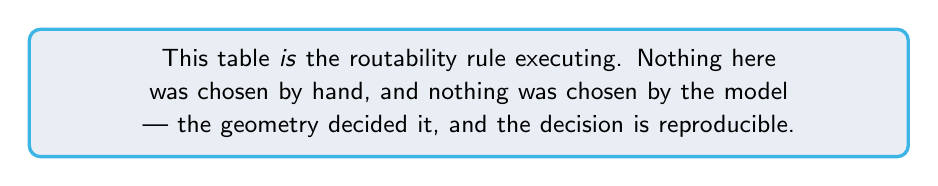
\begin{tikzpicture}
\node[draw=stcyan,very thick,rounded corners=4pt,fill=stlight,inner sep=7pt,align=center,text width=0.88\textwidth]
{\small This table \emph{is} the routability rule executing. Nothing here was chosen by hand, and nothing was chosen by the model ---
the geometry decided it, and the decision is reproducible.};
\end{tikzpicture}
\end{center}
\end{frame}

%-----------------------------------------------------------------------
\begin{frame}{Phase 2 --- layout and routing pipeline (12 stages)}
\vspace{0.5mm}
\begin{center}
\resizebox{\textwidth}{!}{%
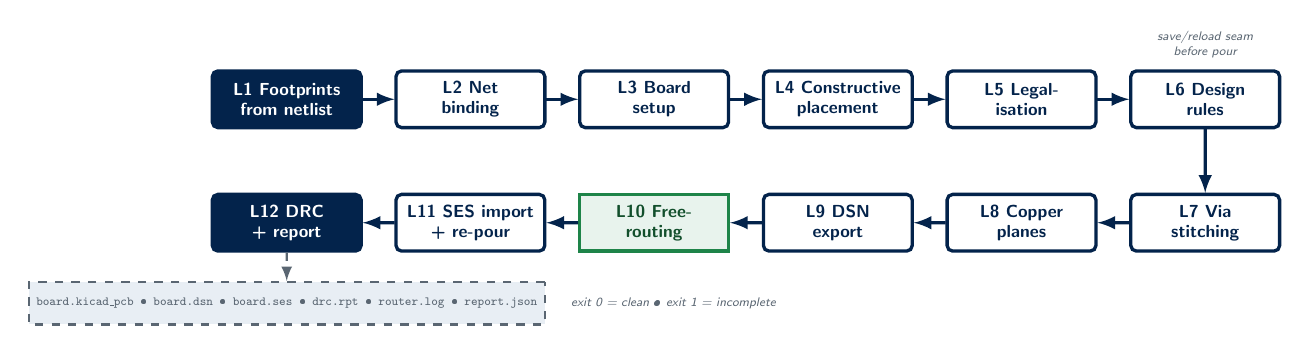
\begin{tikzpicture}[node distance=4.5mm and 4.5mm, scale=0.9, transform shape]
  \node[stgf,minimum width=21mm] (l1) {L1 Footprints\\from netlist};
  \node[stg,right=of l1,minimum width=21mm] (l2) {L2 Net\\binding};
  \node[stg,right=of l2,minimum width=21mm] (l3) {L3 Board\\setup};
  \node[stg,right=of l3,minimum width=21mm] (l4) {L4 Constructive\\placement};
  \node[stg,right=of l4,minimum width=21mm] (l5) {L5 Legal-\\isation};
  \node[stg,right=of l5,minimum width=21mm] (l6) {L6 Design\\rules};

  \node[stg,below=9mm of l6,minimum width=21mm] (l7) {L7 Via\\stitching};
  \node[stg,left=of l7,minimum width=21mm]  (l8) {L8 Copper\\planes};
  \node[stg,left=of l8,minimum width=21mm]  (l9) {L9 DSN\\export};
  \node[ext,left=of l9,minimum width=21mm]  (l10){L10 Free-\\routing};
  \node[stg,left=of l10,minimum width=21mm] (l11){L11 SES import\\+ re-pour};
  \node[stgf,left=of l11,minimum width=21mm](l12){L12 DRC\\+ report};

  \draw[fl] (l1)--(l2); \draw[fl] (l2)--(l3); \draw[fl] (l3)--(l4);
  \draw[fl] (l4)--(l5); \draw[fl] (l5)--(l6);
  \draw[fl] (l6)--(l7);
  \draw[fl] (l7)--(l8); \draw[fl] (l8)--(l9); \draw[fl] (l9)--(l10);
  \draw[fl] (l10)--(l11); \draw[fl] (l11)--(l12);

  \node[art,below=4mm of l12,align=center] (o) {\texttt{board.kicad\_pcb} \textbullet\ \texttt{board.dsn} \textbullet\ \texttt{board.ses} \textbullet\ \texttt{drc.rpt} \textbullet\ \texttt{router.log} \textbullet\ \texttt{report.json}};
  \draw[-latex,thick,stgrey,dashed] (l12)--(o);
  \node[lbl,right=3mm of o] {exit 0 = clean \textbullet\ exit 1 = incomplete};
  \node[lbl,above=1mm of l6,align=center] {save/reload seam\\before pour};
\end{tikzpicture}}
\end{center}
\vspace{2mm}
\begin{center}\footnotesize
\textbf{One command, one timestamped directory.} Netlist in, routed board out --- no GUI, no manual step, machine-readable verdict.
\end{center}
\end{frame}

%-----------------------------------------------------------------------
\begin{frame}{Inside the layout stages}
\vspace{1mm}
\begin{columns}[T]
\begin{column}{0.49\textwidth}
\small
\textbf{Board \& stackup (L3)}
\begin{itemize}\footnotesize
  \item 4-layer stackup; inner layers declared \code{LT\_POWER} (a plane-layer declaration bug cost real DRC accuracy until found)
  \item DFM floors taken from the fab's published spec (PCB Power)
\end{itemize}
\textbf{Placement (L4--L5)}
\begin{itemize}\footnotesize
  \item Constructive placement driven by \textbf{per-edge decap lane assignment}, using the \emph{real ball coordinates} from the WLCSP-72 and LGA-14 footprints
  \item Force-directed legaliser: simultaneous displacement accumulation, stagnation escape by axis-flipping, epsilon convergence \\ ({\itshape converged in 16 iterations})
\end{itemize}
\end{column}
\begin{column}{0.49\textwidth}
\small
\textbf{Design rules (L6)}
\begin{itemize}\footnotesize
  \item Tiered provenance for every constant: \textbf{fab floor} $>$ \textbf{IPC-2221} $>$ \textbf{policy}
  \item 4 netclasses, 68 nets assigned
\end{itemize}
\textbf{Stitching \& pours (L7--L8)}
\begin{itemize}\footnotesize
  \item Via stitching with combined copper \emph{and} hole-clearance geometry
  \item Idempotent zone replacement for the copper pours
\end{itemize}
\textbf{Routing bridge (L9--L11)}
\begin{itemize}\footnotesize
  \item Native \code{ExportSpecctraDSN} / \code{ImportSpecctraSES}
  \item Freerouting invoked headless as a subprocess
\end{itemize}
\end{column}
\end{columns}
\end{frame}

%-----------------------------------------------------------------------
\begin{frame}{The derived router clearance --- a worked example}
\vspace{0mm}
\begin{block}{Problem}
\small
The DSN format carries \textbf{copper-to-copper} clearance. It does \textbf{not} carry KiCad's \textbf{hole-to-copper} rule --- so a router that satisfies the DSN can still produce a board that fails KiCad's DRC.
\end{block}
\vspace{1mm}
\begin{block}{Solution --- inflate the exported clearance so one rule implies the other}
\vspace{1mm}
\begin{center}\large
$c_{\text{router}} \;=\; \max\bigl(c_{\text{copper}},\; c_{\text{hole}} + r_{\text{hole}} - r_{\text{via}}\bigr) \;=\; \mathbf{0.1250\ mm}$
\end{center}
\vspace{1mm}
\small
Satisfying copper-to-copper at 0.1250\,mm now \emph{automatically} satisfies hole-to-copper. Applied \textbf{in memory} with immediate revert --- netclass definitions live in \code{.kicad\_pro} and do not survive a save/reload round-trip.
\end{block}
\vspace{1mm}
\begin{center}\footnotesize
\textbf{And the number was measured, not chosen:} \quad
0.09\,mm $\rightarrow$ 6 unrouted, \alert{14 hole violations} \quad\textbullet\quad
\textbf{0.1250\,mm $\rightarrow$ 10 unrouted, 0 violations}
\end{center}
\vspace{1mm}
\begin{center}\footnotesize\color{stgrey}
The shape of most of the engineering here: not "call the API", but \emph{find the semantic gap between two tools and close it with a derivation you can defend}.
\end{center}
\end{frame}

%-----------------------------------------------------------------------
\begin{frame}{Output 2 --- the board that comes out}
\vspace{1mm}
\begin{columns}[T]
\begin{column}{0.51\textwidth}
\begin{center}\footnotesize
\begin{tabular}{@{}l l@{}}
\toprule
\textbf{Property} & \textbf{Value}\\
\midrule
Board area & $\approx$ 625 mm$^2$\\
Layers & 4 (inner = \code{LT\_POWER})\\
Assembly & single-sided\\
Copper pour, layer 4 & GND\\
Copper pour, layer 6 & \code{/VDD\_3V3}\\
Stitching vias & 40 placed, 1 unreachable\\
Traces after routing & 94\\
Vias, total & 44\\
Router clearance & 0.1250 mm derived\\
Fab floor clearance & 0.09 mm\\
\bottomrule
\end{tabular}
\end{center}
\end{column}
\begin{column}{0.45\textwidth}
\begin{block}{What the placer actually did}
\small
Read the real ball coordinates out of the WLCSP-72 and LGA-14 footprints, assigned each decoupling capacitor to a lane on the edge of U1 nearest its own supply ball, then let the force-directed legaliser resolve the overlaps.\\[3pt]
It converged in \textbf{16 iterations}.
\end{block}
\vspace{1mm}
\begin{block}{What it did not do}
\small
\gap\ No bottom-side placement --- the placer has no concept of a second side.\\[3pt]
\gap\ No intentional trace widths --- see Part 3.
\end{block}
\end{column}
\end{columns}
\end{frame}

%-----------------------------------------------------------------------
\begin{frame}[fragile]{Output 3 --- the machine-readable verdict}
\vspace{1mm}
\begin{columns}[T]
\begin{column}{0.55\textwidth}
\begin{lstlisting}
>>> [L1/12] Footprints from netlist
    components: 22 | nets: 68 | pads: 126
>>> [L5/12] Legalization
    converged in 16 iterations
>>> [L6/12] Design rules
    classes: 4 | nets assigned: 68
>>> [L7/12] Via stitching
    stitched: 40 | unstitched: 1
      UNREACHABLE U1 pad H8 (/VDD_3V3)
>>> [L8/12] Copper planes
      poured GND on layer 4
      poured /VDD_3V3 on layer 6
>>> [L9/12] DSN export
    router clearance: 0.1250 mm
>>> [L10/12] Autorouting
    router ok: True | unrouted: 10
>>> [L11/12] SES import + re-pour
    traces: 94 | vias: 44
>>> [L12/12] DRC
    unconnected: 10 | copper: 0 | silk: 10
=== INCOMPLETE ===   exit code: 1
\end{lstlisting}
\end{column}
\begin{column}{0.43\textwidth}
\begin{block}{Honest failure is a feature}
\small
The run above is a \textbf{correct} result, not a regression.\\[4pt]
10 unconnected items means the board is \emph{not} clean --- so the pipeline says \code{INCOMPLETE} and returns \code{exit 1}.
\end{block}
\vspace{2mm}
\begin{block}{Why this matters}
\small
A flow that reports success optimistically is worse than no automation: it moves error discovery to the fab.\\[4pt]
Every stage either proves its result or names what it could not do (\code{UNREACHABLE U1 pad H8}).
\end{block}
\end{column}
\end{columns}
\end{frame}

%-----------------------------------------------------------------------
\begin{frame}{Where we stand --- the scorecard}
\vspace{1mm}
\begin{center}\small
\begin{tabular}{@{}p{0.40\textwidth} p{0.30\textwidth} c@{}}
\toprule
\textbf{Metric} & \textbf{Result} & \textbf{Status}\\
\midrule
ERC errors (schematic) & 0 & \ok\\
Independent verifier & clean & \ok\\
Components / nets / pads & 22 / 68 / 126 & \ok\\
Pads bound to nets & 126 / 126 & \ok\\
Courtyard violations & 0 & \ok\\
Copper clearance violations & 0 & \ok\\
Via stitching & 40 placed, 1 named unreachable & \gap\\
Unconnected items & 10 (measured trade for 0 violations) & \gap\\
Silkscreen warnings & 10 (deferred, cosmetic) & \gap\\
Manual/GUI steps required & 0 & \ok\\
\bottomrule
\end{tabular}
\end{center}
\vspace{3mm}
\begin{center}\footnotesize
\textbf{Phase 1 complete.} \quad \textbf{Phase 2 complete as a pipeline}, with a named, understood residual: the WLCSP-72 inner-ball fan-out.
\end{center}
\end{frame}

%=======================================================================
\section{Part 2 --- Replicating the work}
%=======================================================================
{\setbeamercolor{background canvas}{bg=stblue}
\begin{frame}[plain]
\vfill
\begin{center}
{\color{stcyan}\Large\textbf{Part 2}}\\[6pt]
{\color{white}\LARGE\textbf{Replicating the work}}\\[10pt]
{\color{white}\small Environment, dependencies, SKiDL, KiCad, Freerouting, LLM APIs}\\[4pt]
{\color{stcyan}\footnotesize 15 minutes}
\end{center}
\vfill
\end{frame}}

%-----------------------------------------------------------------------
\begin{frame}{The environment split --- and why it exists}
\vspace{1mm}
\begin{center}
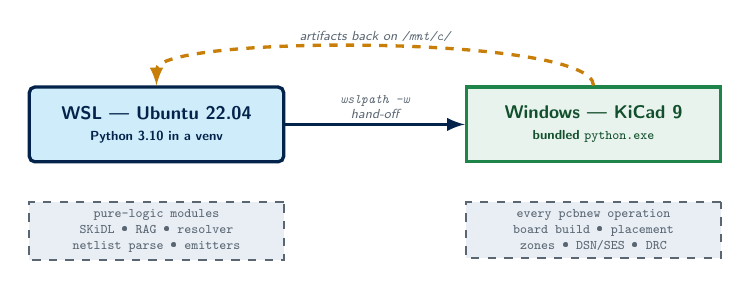
\begin{tikzpicture}[node distance=6mm and 10mm, scale=0.95, transform shape]
  \node[stgc,minimum width=34mm,minimum height=10mm] (wsl) {\textbf{WSL --- Ubuntu 22.04}\\{\tiny Python 3.10 in a venv}};
  \node[art,below=5mm of wsl,minimum width=34mm,align=center] (wm)
    {pure-logic modules\\SKiDL \textbullet\ RAG \textbullet\ resolver\\ netlist parse \textbullet\ emitters};
  \node[ext,right=24mm of wsl,minimum width=34mm,minimum height=10mm] (win) {\textbf{Windows --- KiCad 9}\\{\tiny bundled \texttt{python.exe}}};
  \node[art,below=5mm of win,minimum width=34mm,align=center] (winm)
    {every \texttt{pcbnew} operation\\board build \textbullet\ placement\\ zones \textbullet\ DSN/SES \textbullet\ DRC};
  \draw[fl] (wsl)--(win) node[lbl,midway,above,align=center] {\texttt{wslpath -w}\\hand-off};
  \draw[flb] (win) .. controls +(0,12mm) and +(0,12mm) .. (wsl)
        node[lbl,midway,above] {artifacts back on \texttt{/mnt/c/}};
\end{tikzpicture}
\end{center}
\vspace{2mm}
\begin{columns}[T]
\begin{column}{0.52\textwidth}
\begin{block}{Why not one machine?}
\small
\code{pcbnew} is a SWIG binding into KiCad's C++ core. It must run under the \emph{same} interpreter KiCad ships. Mixing it with a Linux venv gives ABI mismatches that fail in confusing ways.
\end{block}
\end{column}
\begin{column}{0.45\textwidth}
\begin{block}{Practical rule}
\small
Anything that is \emph{pure logic} $\rightarrow$ WSL Python.\\
Anything that \emph{touches a board object} $\rightarrow$ KiCad's Windows \code{python.exe}.
\end{block}
\end{column}
\end{columns}
\end{frame}

%-----------------------------------------------------------------------
\begin{frame}[fragile]{Step 1 --- base environment}
\vspace{1mm}
\textbf{A. WSL + Python}
\begin{lstlisting}
wsl --install -d Ubuntu-22.04          # from Windows PowerShell
sudo apt update && sudo apt install -y python3.10 python3.10-venv python3-pip git

mkdir -p ~/LLM_Driven_Schematic_Gen && cd ~/LLM_Driven_Schematic_Gen
python3 -m venv venv
source venv/bin/activate
python -V                              # expect: Python 3.10.x
\end{lstlisting}
\vspace{1mm}
\textbf{B. KiCad 9 on the Windows side}
\begin{lstlisting}
# install KiCad 9.0 from kicad.org (Windows installer)
# then verify the symbol libraries are visible from WSL:
ls "/mnt/c/Program Files/KiCad/9.0/share/kicad/symbols/" | head
"/mnt/c/Program Files/KiCad/9.0/bin/python.exe" -c "import pcbnew; print(pcbnew.Version())"
\end{lstlisting}
\vspace{1mm}
\begin{center}\footnotesize\color{stred}
The install path contains a space --- \textbf{always quote it}. Unquoted, it fails silently in half of all shell contexts.
\end{center}
\end{frame}

%-----------------------------------------------------------------------
\begin{frame}[fragile]{Step 2 --- Python dependencies}
\vspace{-1mm}
\begin{lstlisting}
source ~/LLM_Driven_Schematic_Gen/venv/bin/activate

# --- netlist generation -----------------------------------
pip install skidl==2.2.3           # Python -> netlist + ERC()
pip install anthropic==0.115.1     # primary LLM provider
pip install openai==2.46.0         # NVIDIA NIM (OpenAI-compatible)

# --- retrieval-augmented grounding -------------------------
pip install pymupdf4llm==1.28.0    # layout-aware PDF -> markdown
pip install pymupdf-layout==1.28.0
pip install chromadb==1.5.9        # vector store
pip install sentence-transformers==5.6.0

pip freeze > requirements.txt      # these are the tested pins
\end{lstlisting}
\vspace{-1mm}
\begin{columns}[T]
\begin{column}{0.49\textwidth}
\begin{block}{Do not skip \code{pymupdf4llm}}
\small
Plain PyMuPDF turns the STM32 ball-assignment tables into mojibake. The model is then grounded on garbage, and the failure surfaces three stages later as an invalid pin name.
\end{block}
\end{column}
\begin{column}{0.49\textwidth}
\begin{block}{SKiDL's role}
\small
SKiDL is the \emph{intermediate representation}: the LLM writes Python; SKiDL executes it into a netlist and runs \code{ERC()}. The LLM never writes a file format.
\end{block}
\end{column}
\end{columns}
\end{frame}

%-----------------------------------------------------------------------
\begin{frame}[fragile]{Step 3 --- Freerouting and Java}
\vspace{1mm}
\begin{lstlisting}
# Windows side: install a JRE, then confirm
java -version

# place the Freerouting jar somewhere stable, e.g.
#   C:\tools\freerouting\freerouting.jar

# the pipeline invokes it headless as a subprocess:
java -jar freerouting.jar -de board.dsn -do board.ses
\end{lstlisting}
\vspace{2mm}
\begin{columns}[T]
\begin{column}{0.52\textwidth}
\begin{block}{The bridge is pcbnew-native}
\small
KiCad 9 exposes both halves in Python --- \code{pcbnew.ExportSpecctraDSN} and \code{pcbnew.ImportSpecctraSES}.\\[3pt]
No GUI export step: \code{board $\rightarrow$ DSN $\rightarrow$ Freerouting $\rightarrow$ SES $\rightarrow$ board $\rightarrow$ DRC}.
\end{block}
\end{column}
\begin{column}{0.45\textwidth}
\begin{block}{Verify before you trust}
\small
Check the JRE version your Freerouting build requires --- recent releases track new JREs and fail with an opaque error on older ones.
\end{block}
\end{column}
\end{columns}
\end{frame}

%-----------------------------------------------------------------------
\begin{frame}[fragile]{Step 4 --- LLM API configuration}
\vspace{1mm}
\textbf{Provider A --- Anthropic (baseline)}
\begin{lstlisting}
export ANTHROPIC_API_KEY=sk-ant-...     # from console.anthropic.com
# MODEL      = "claude-sonnet-4-6"
# max_tokens = 4000
\end{lstlisting}
\textbf{Provider B --- NVIDIA NIM (OpenAI-compatible, free tier)}
\begin{lstlisting}
export NVIDIA_API_KEY=nvapi-...         # from build.nvidia.com
# base_url = "https://integrate.api.nvidia.com/v1"
# model    = "z-ai/glm-5.2"
# temperature low + fixed seed for reproducible codegen
\end{lstlisting}
\vspace{1mm}
\begin{columns}[T]
\begin{column}{0.52\textwidth}
\begin{block}{One switch, not a migration}
\small
A single \code{PROVIDER} flag selects the branch. Both branches return \code{(text, in\_tokens, out\_tokens)}, so everything downstream --- including the cost log --- stays provider-neutral.
\end{block}
\end{column}
\begin{column}{0.45\textwidth}
\begin{block}{Two things people get wrong}
\small
\begin{itemize}\footnotesize
  \item A \textbf{Claude Pro subscription is not API access} --- the API bills separately.
  \item The sample \code{temperature=1} in most quickstarts is wrong for code generation.
\end{itemize}
\end{block}
\end{column}
\end{columns}
\end{frame}

%-----------------------------------------------------------------------
\begin{frame}[fragile]{Step 5 --- run the flow}
\vspace{1mm}
\textbf{Build the RAG index (once per datasheet set)}
\begin{lstlisting}
source ~/LLM_Driven_Schematic_Gen/venv/bin/activate
cd ~/LLM_Driven_Schematic_Gen/rag
python build_rag_v2.py            # pymupdf4llm extract -> chunk -> embed -> Chroma
\end{lstlisting}
\textbf{Phase 1 --- prompt to verified schematic (one command)}
\begin{lstlisting}
python pipeline.py --name spi_auto --output-root /mnt/c/.../pcbgen_outputs
python pipeline.py --name spi_auto --skip-generate   # re-serialise, no tokens
\end{lstlisting}
\textbf{Phase 2 --- netlist to routed board (KiCad's Windows Python)}
\begin{lstlisting}
"/mnt/c/Program Files/KiCad/9.0/bin/python.exe" \
  "$(wslpath -w ~/LLM_Driven_Schematic_Gen/rag/layout_pipeline.py)" \
  'C:\...\joined_e2e\joined_e2e.net'  "$(wslpath -w $RUN_DIR)"
echo "exit code: $?"               # 0 = clean, 1 = incomplete
\end{lstlisting}
\vspace{1mm}
\begin{center}\footnotesize\color{stgrey}
Phase 1 runs entirely in the venv. Phase 2 must be launched with KiCad's own interpreter --- never the venv Python.
\end{center}
\end{frame}

%-----------------------------------------------------------------------
\begin{frame}{Verified environment --- the tested combination}
\vspace{-1mm}
\begin{columns}[T]
\begin{column}{0.50\textwidth}
\begin{center}\footnotesize
\begin{tabular}{@{}l r@{}}
\toprule
\textbf{Component} & \textbf{Version}\\
\midrule
KiCad / \code{pcbnew} & \textbf{9.0.8}\\
OS & Ubuntu 22.04 (WSL)\\
Python & 3.10\\
\midrule
\code{skidl} & 2.2.3\\
\code{anthropic} & 0.115.1\\
\code{openai} & 2.46.0\\
\code{pymupdf} & 1.28.0\\
\code{pymupdf-layout} & 1.28.0\\
\code{pymupdf4llm} & 1.28.0\\
\code{chromadb} & 1.5.9\\
\code{sentence-transformers} & 5.6.0\\
\bottomrule
\end{tabular}
\end{center}
\end{column}
\begin{column}{0.47\textwidth}
\begin{block}{Why pin all of it}
\small
\code{pcbnew} is a SWIG binding to a specific KiCad build. A minor KiCad bump can change enum names, default clearances, or whether a call exists at all --- and the failure shows up as a wrong \emph{number}, not an exception.
\end{block}
\vspace{1mm}
\begin{block}{Still unpinned --- to close before publication}
\small
\begin{itemize}\footnotesize
  \item \gap\ Freerouting jar version
  \item \gap\ JRE version on the Windows side
  \item \gap\ Fab DFM spec revision (PCB Power)
\end{itemize}
Each of these silently changes results. They belong in \code{report.json}, recorded per run.
\end{block}
\end{column}
\end{columns}
\end{frame}

%-----------------------------------------------------------------------
\begin{frame}{Module map --- the real repository}
\vspace{-2mm}
\begin{center}\scriptsize
\begin{tabular}{@{}p{0.13\textwidth} p{0.52\textwidth} p{0.28\textwidth}@{}}
\toprule
\textbf{Layer} & \textbf{Modules} & \textbf{Responsibility}\\
\midrule
Grounding &
\texttt{build\_rag\_v2} \texttt{query\_rag} \texttt{kicad\_symbol\_parser} \texttt{symbol\_resolver} &
Retrieval; parse \texttt{.kicad\_sym}; authoritative pin table\\
\addlinespace
Generation &
\texttt{generate\_spi\_v2} \texttt{generate\_st\_circuit} \texttt{generate\_i2c\_circuit}\newline
\texttt{lsm6dsm\_stm32l476\_spi\_v2} \emph{(generated)} \textbullet\ \texttt{...CLAUDE\_BASELINE} \emph{(frozen known-good)} &
Prompt assembly, provider switch, SKiDL codegen, ERC gate\\
\addlinespace
Schematic &
\texttt{netlist\_parser} \texttt{netlist\_reader} \texttt{component\_model} \texttt{geometry}\newline
\texttt{grouping} \texttt{roles} \texttt{placement} \texttt{power\_wiring}\newline
\texttt{schematic\_emitter} \texttt{kicad\_sch\_builder} \texttt{kicad\_sch\_writer} \texttt{pipeline} &
Netlist $\rightarrow$ geometry $\rightarrow$ ST-style power wiring $\rightarrow$ \texttt{.kicad\_sch}\\
\addlinespace
Verification &
\texttt{verify\_schematic} \textbullet\ 6 $\times$ \texttt{check\_*} &
Union-find on drawn connectivity; clearance audits\\
\addlinespace
Layout &
\texttt{board\_setup} \texttt{board\_builder} \texttt{placement\_engine} \texttt{legalize}\newline
\texttt{design\_rules} \texttt{rules\_apply} \texttt{via\_stitch} \texttt{via\_geom} \texttt{zones}\newline
\texttt{export\_dsn} \texttt{routing} \texttt{analyze\_ses} \texttt{layout\_pipeline} \texttt{run\_context} &
Placement, rules, stitching, pours, DSN/SES bridge, DRC + report\\
\bottomrule
\end{tabular}
\end{center}
\vspace{0.5mm}
\begin{center}\scriptsize
Plus harnesses: \texttt{layout\_stage2..12\_*.py} per-stage runners \textbullet\ \textbf{13} \texttt{probe\_*.py} \textbullet\ \textbf{7} \texttt{test\_*.py}
\end{center}
\end{frame}

%-----------------------------------------------------------------------
\begin{frame}{The 13 probe scripts --- discipline made visible}
\vspace{1mm}
\begin{columns}[T]
\begin{column}{0.56\textwidth}
\small Each \code{probe\_*.py} is a question asked of the tooling \textbf{before} any code was written against it:
\vspace{1mm}
\begin{center}\scriptsize
\begin{tabular}{@{}p{0.42\textwidth} p{0.52\textwidth}@{}}
\texttt{layertype} & can I declare a plane layer?\\
\texttt{netclass\_api} & does the API expose netclasses?\\
\texttt{netclass\_assign} & does assignment stick?\\
\texttt{roundtrip\_nc} & does it survive save/reload?\\
\texttt{zone} \textbullet\ \texttt{pour\_inmem} & can I pour in memory?\\
\texttt{inmem\_courtyard} & is courtyard data live?\\
\texttt{via} \textbullet\ \texttt{via\_in\_pad} & what via geometry is legal?\\
\texttt{ses\_import} & does import preserve prior work?\\
\texttt{java\_subprocess} & can I drive Freerouting headless?\\
\texttt{clearance\_cost} & what does clearance cost me?\\
\texttt{cachefix} & is the symbol cache stale?\\
\end{tabular}
\end{center}
\end{column}
\begin{column}{0.41\textwidth}
\begin{block}{The rule behind them}
\small
\textbf{Never write final code against an assumption} about a library API, tool output, or environment state. Probe first; build on the confirmed result.
\end{block}
\vspace{1mm}
\begin{block}{What it bought}
\small
\code{roundtrip\_netclass} is why we know netclasses live in the \code{.kicad\_pro} file.\\[3pt]
\code{pour\_inmem} is why the save/reload seam exists instead of a mysterious C++ crash.\\[4pt]
\textbf{Each probe is a bug that never happened.}
\end{block}
\end{column}
\end{columns}
\end{frame}

%-----------------------------------------------------------------------
\begin{frame}{Gotchas that cost real time --- read before you build}
\vspace{1mm}
\begin{center}\scriptsize
\begin{tabular}{@{}p{0.36\textwidth} p{0.58\textwidth}@{}}
\toprule
\textbf{Trap} & \textbf{What actually happens / the fix}\\
\midrule
\textbf{Stale \texttt{.kicad\_pro}} &
KiCad 9 stores \emph{netclass definitions in the project file}, not the board. \texttt{SaveBoard} will not overwrite an existing \texttt{.kicad\_pro}, so a stale file silently overrides your computed design rules and invalidates every measurement. \textbf{Delete it before saving.}\\
\addlinespace
\textbf{Netclass round-trip} &
Netclasses do not survive save $\rightarrow$ reload through a temp path. Do the DSN clearance inflation \textbf{in memory}, with an immediate revert.\\
\addlinespace
\textbf{\texttt{ZONE\_FILLER} crash} &
Hard-crashes at the C++ level on an in-memory board, with \emph{no Python traceback}. \texttt{BuildConnectivity()} does not help. Insert a deliberate \textbf{save/reload seam before pouring}.\\
\addlinespace
\textbf{Plane layer type} &
Inner layers must be declared \texttt{LT\_POWER}, or the DRC engine reports misleading clearance results.\\
\addlinespace
\textbf{Path with a space} &
\texttt{C:\textbackslash Program Files\textbackslash KiCad\textbackslash 9.0} --- quote it everywhere, and use \texttt{wslpath -w} for every hand-off.\\
\addlinespace
\textbf{Unsourced constants} &
A \texttt{POWER} clearance of 0.15\,mm was invented, not sourced. Removing it and grounding to the fab floor (0.09\,mm) \textbf{recovered four connections}. \emph{No unsourced constants in a release.}\\
\bottomrule
\end{tabular}
\end{center}
\end{frame}

%-----------------------------------------------------------------------
\begin{frame}{Reproducibility}
\vspace{2mm}
\begin{columns}[T]
\begin{column}{0.49\textwidth}
\textbf{What is already deterministic}
\begin{itemize}\small
  \item Every run writes to a \textbf{timestamped directory} with all six artifacts.
  \item \code{report.json} records stage-by-stage results, not just the final verdict.
  \item Exit code carries the verdict: \code{0} clean, \code{1} incomplete.
  \item The legaliser converges to an epsilon, not a fixed iteration count --- same input, same output.
\end{itemize}
\end{column}
\begin{column}{0.49\textwidth}
\textbf{What still varies}
\begin{itemize}\small
  \item \gap\ The LLM stage. Anthropic's API exposes no seed; NVIDIA NIM does --- so GLM runs are \emph{more} reproducible than the Claude baseline.
  \item \gap\ Freerouting is heuristic; different runs may route differently, though the DRC verdict has been stable.
\end{itemize}
\vspace{2mm}
\begin{block}{Publication checklist}
\small
Pin \code{requirements.txt}; record KiCad build, Freerouting version, JRE version, model ID and temperature/seed \emph{in} \code{report.json}.
\end{block}
\end{column}
\end{columns}
\end{frame}

%=======================================================================
\section{Part 3 --- Next tasks}
%=======================================================================
{\setbeamercolor{background canvas}{bg=stblue}
\begin{frame}[plain]
\vfill
\begin{center}
{\color{stcyan}\Large\textbf{Part 3}}\\[6pt]
{\color{white}\LARGE\textbf{Next tasks}}\\[10pt]
{\color{white}\small Open gaps, the release bar, and the north star}\\[4pt]
{\color{stcyan}\footnotesize 15 minutes}
\end{center}
\vfill
\end{frame}}

%-----------------------------------------------------------------------
\begin{frame}{Roadmap}
\vspace{2mm}
\begin{center}
\resizebox{\textwidth}{!}{%
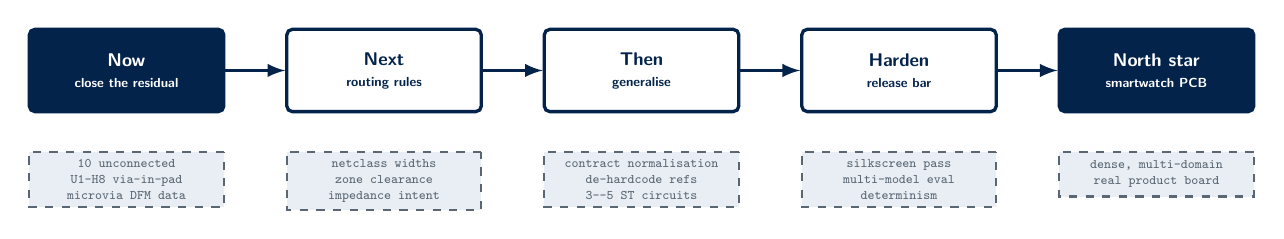
\begin{tikzpicture}[node distance=6mm and 8mm, scale=0.95, transform shape]
  \node[stgf,minimum width=26mm,minimum height=11mm] (n1) {\textbf{Now}\\{\tiny close the residual}};
  \node[stg,right=of n1,minimum width=26mm,minimum height=11mm] (n2) {\textbf{Next}\\{\tiny routing rules}};
  \node[stg,right=of n2,minimum width=26mm,minimum height=11mm] (n3) {\textbf{Then}\\{\tiny generalise}};
  \node[stg,right=of n3,minimum width=26mm,minimum height=11mm] (n4) {\textbf{Harden}\\{\tiny release bar}};
  \node[stgf,right=of n4,minimum width=26mm,minimum height=11mm] (n5) {\textbf{North star}\\{\tiny smartwatch PCB}};
  \draw[fl] (n1)--(n2); \draw[fl] (n2)--(n3); \draw[fl] (n3)--(n4); \draw[fl] (n4)--(n5);

  \node[art,below=5mm of n1,minimum width=26mm] {10 unconnected\\U1-H8 via-in-pad\\microvia DFM data};
  \node[art,below=5mm of n2,minimum width=26mm] {netclass widths\\zone clearance\\impedance intent};
  \node[art,below=5mm of n3,minimum width=26mm] {contract normalisation\\de-hardcode refs\\3--5 ST circuits};
  \node[art,below=5mm of n4,minimum width=26mm] {silkscreen pass\\multi-model eval\\determinism};
  \node[art,below=5mm of n5,minimum width=26mm] {dense, multi-domain\\real product board};
\end{tikzpicture}}
\end{center}
\end{frame}

%-----------------------------------------------------------------------
\begin{frame}{Task 1 --- close the 10 unconnected}
\vspace{-2mm}
\begin{columns}[T]
\begin{column}{0.52\textwidth}
\textbf{Root cause}\\[2pt]
\small All ten are \textbf{WLCSP-72 inner-ball escape routes}. At 0.4\,mm ball pitch, the keep-out ring leaves no legal channel for a through-via to reach U1's inner balls.
\vspace{1mm}

\textbf{We already know the price of the alternative}
\begin{center}\scriptsize
\begin{tabular}{@{}l c c@{}}
\toprule
\textbf{Router clearance} & \textbf{Unrouted} & \textbf{Hole violations}\\
\midrule
0.09 mm & 6 & \alert{14}\\
\textbf{0.1250 mm} & \textbf{10} & \textbf{0}\\
\bottomrule
\end{tabular}
\end{center}
\vspace{1mm}

\textbf{The plan}
\begin{itemize}\small
  \item \textbf{Via-in-pad} for \code{U1-H8} --- geometry proven: a 0.225\,mm pad permits a via up to 0.395\,mm.
  \item Choose the via strategy \emph{explicitly}: microvia / blind-buried vs. through.
  \item \gap\ \textbf{Blocked}: awaiting the fab's microvia drill, annular ring and hole-clearance specs.
\end{itemize}
\end{column}
\begin{column}{0.45\textwidth}
\begin{block}{The general principle}
\small
Fine-pitch BGA and WLCSP escape is a \textbf{stackup decision, not a router decision}. No autorouter can solve a fan-out that the layer count forbids --- the options are more layers, microvias, or unused balls.
\end{block}
\vspace{1mm}
\begin{block}{Why this is the right first task}
\small
The 0.09\,mm board connects four more nets and is \textbf{not manufacturable}. We took the manufacturable one.\\[3pt]
Not a bug --- but it is the only thing between this run and \code{exit 0}, and closing it means changing the \emph{stackup}.
\end{block}
\end{column}
\end{columns}
\end{frame}

%-----------------------------------------------------------------------
\begin{frame}{Task 2 --- routing rules: the honest gap}
\vspace{2mm}
\begin{block}{Self-assessment}
\small
We set \code{m\_TrackMinWidth = 0.09\,mm} --- but that is a \textbf{minimum the DRC enforces}, not the width the \textbf{router uses}.
We never created netclasses with actual widths, so Freerouting routed at the DSN default.\\[4pt]
\textbf{Every trace on the current board is a width nobody specified.} Zone clearance had the same problem --- it sat at KiCad's unsourced 0.5\,mm default until it was grounded to the fab floor. Trace widths are the last one left.
\end{block}
\vspace{2mm}
\begin{columns}[T]
\begin{column}{0.49\textwidth}
\textbf{What to build}
\begin{itemize}\small
  \item Real netclasses with \emph{intentional} widths per class: power / ground / signal / high-speed.
  \item Current-carrying width from IPC-2221 for the supply rails.
  \item Explicit zone local clearance --- no inherited defaults.
\end{itemize}
\end{column}
\begin{column}{0.49\textwidth}
\textbf{What comes after}
\begin{itemize}\small
  \item Length matching and impedance intent for the SPI bus (not needed at these speeds --- needed for the north star).
  \item Differential-pair support.
  \item Per-class via rules.
\end{itemize}
\end{column}
\end{columns}
\end{frame}

%-----------------------------------------------------------------------
\begin{frame}{Task 3 --- generalisation}
\vspace{1mm}
\begin{columns}[T]
\begin{column}{0.49\textwidth}
\begin{block}{Generation-contract normalisation}
\small
The multi-model experiment proved the pipeline is brittle to naming variants:\\[3pt]
\code{VSS} vs \code{GND} \textbullet\ \code{VDD} vs \code{VDD\_3V3} \textbullet\ \code{VREF+} vs \code{VREF\_PLUS} \textbullet\ \code{100n} vs \code{100nF}\\[3pt]
Add a normalisation layer so layout never breaks on off-contract input.
\end{block}
\vspace{1mm}
\begin{block}{De-hardcode the placer}
\small
Circuit-specific reference designators (the \code{R3}/\code{R4}-style hardcodes) must go. The layout stage has to be \textbf{topology-agnostic} to be a product.
\end{block}
\end{column}
\begin{column}{0.49\textwidth}
\begin{block}{Broaden the benchmark}
\small
Prove the full flow on \textbf{3--5 diverse ST circuits}, not one board. First addition: an STM32F0 motor-controller topology --- different package, different rail structure, different constraints.
\end{block}
\vspace{1mm}
\begin{block}{Double-sided placement}
\small
Today every component is top-side; the placer has \textbf{no concept of a bottom side}. Real designers push passives to the solder side when the top crowds. Needs per-side collision sets and \code{B.CrtYd} courtyards.
\end{block}
\end{column}
\end{columns}
\end{frame}

%-----------------------------------------------------------------------
\begin{frame}{Task 4 --- multi-model evaluation}
\vspace{0.5mm}
\small
A controlled comparison: identical prompt, identical RAG context, different model.
\vspace{1mm}
\begin{center}\small
\begin{tabular}{@{}p{0.28\textwidth} p{0.62\textwidth}@{}}
\toprule
\textbf{Observation} & \textbf{Detail}\\
\midrule
Format contract held & GLM-5.2 produced valid SKiDL Python, no markdown leakage \ok\\
\addlinespace
ERC-invisible pin error & A signal pin was mis-named: syntactically valid, electrically wrong. \textbf{ERC did not catch it.} \no\\
\addlinespace
Off-contract net names & \code{VSS}/\code{VDD}/\code{VREF+} instead of the contract --- broke the power-wiring stage \no\\
\addlinespace
Missing components & Absent resistors tripped the placement hardcodes \no\\
\bottomrule
\end{tabular}
\end{center}
\vspace{1mm}
\begin{block}{Conclusion}
\small
\textbf{Multi-model validation is not optional} --- a single model's idiosyncrasies get silently encoded into the pipeline's assumptions. This also gives the first dataset for a paper: \emph{which classes of hardware error survive ERC?}
\end{block}
\end{frame}

%-----------------------------------------------------------------------
\begin{frame}{Definition of done --- the release bar}
\vspace{2mm}
\begin{block}{Layout stage is release-ready when \emph{all} of these hold, across the benchmark set}
\vspace{1mm}
\begin{columns}[T]
\begin{column}{0.48\textwidth}
\begin{itemize}\small
  \item One command: any Phase-1 schematic $\rightarrow$ routed board
  \item \textbf{0 unconnected}
  \item DRC-clean (copper, courtyard, silkscreen)
  \item No unsourced constants anywhere
\end{itemize}
\end{column}
\begin{column}{0.48\textwidth}
\begin{itemize}\small
  \item No GUI steps
  \item No hardcoded reference designators
  \item A clear machine-readable pass/fail report
  \item Deterministic, with honest failure behaviour
\end{itemize}
\end{column}
\end{columns}
\end{block}
\vspace{3mm}
\begin{center}

\begin{tikzpicture}
\node[draw=stcyan,very thick,rounded corners=4pt,fill=stlight,inner sep=8pt,align=center,text width=0.85\textwidth]
{\small\textbf{Acceptance gate, unchanged since Phase 1:} every board must pass \emph{two independent judges} ---\\
KiCad's own DRC \textbf{and} our independent verifier. Neither alone is trusted.};
\end{tikzpicture}
\end{center}
\end{frame}

%-----------------------------------------------------------------------
\begin{frame}{North star --- and what it demands}
\vspace{1mm}
\begin{columns}[T]
\begin{column}{0.50\textwidth}
\textbf{The target: a smartwatch PCB}
\vspace{2mm}
\small Chosen deliberately, because it breaks every simplifying assumption the current pipeline makes:
\begin{itemize}\small
  \item Dense, irregular board outline --- not a rectangle
  \item Multi-domain power: charger, PMIC, multiple rails
  \item Mixed signal: RF, analogue sensors, digital bus
  \item Genuine two-sided assembly
  \item Fine-pitch escape everywhere, not just at U1
\end{itemize}
\end{column}
\begin{column}{0.47\textwidth}
\begin{block}{Asks from ST}
\small
\begin{itemize}\footnotesize
  \item Footprint mappings for the target part families
  \item Recommended stackups
  \item Placement guidelines / checklists
  \item \code{.kicad\_dru} rule files, if they exist
  \item 2--3 reference boards as ground truth
\end{itemize}
\end{block}
\vspace{1mm}
\begin{block}{Open question for discussion}
\small
Where should the LLM's authority end? Today it proposes only the \emph{netlist}. Should it also propose \emph{placement intent} --- or does that break the verifiability that makes this flow trustworthy?
\end{block}
\end{column}
\end{columns}
\end{frame}

%-----------------------------------------------------------------------
\begin{frame}{Summary}
\vspace{2mm}
\begin{columns}[T]
\begin{column}{0.48\textwidth}
\begin{block}{What exists today}
\small
\begin{itemize}\footnotesize
  \item A working, headless, prompt-to-board pipeline for an ST benchmark circuit
  \item 0 ERC errors; 126/126 pads bound; 0 copper and courtyard violations
  \item Two-judge verification catching faults ERC cannot see
  \item Machine-readable reporting with honest failure
\end{itemize}
\end{block}
\end{column}
\begin{column}{0.48\textwidth}
\begin{block}{What is left}
\small
\begin{itemize}\footnotesize
  \item 10 unconnected --- a stackup decision, blocked on fab data
  \item Intentional routing rules (widths, clearances)
  \item Generalisation across circuits and models
  \item Silkscreen, double-sided placement, determinism
\end{itemize}
\end{block}
\end{column}
\end{columns}
\vspace{3mm}
\begin{center}
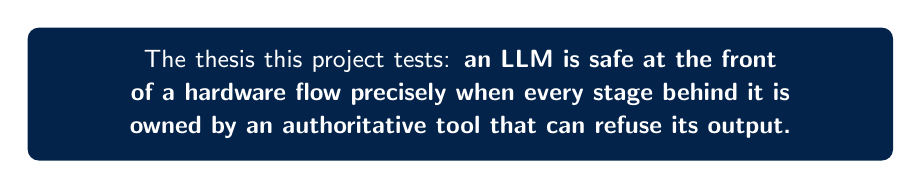
\begin{tikzpicture}
\node[fill=stblue,text=white,rounded corners=4pt,inner sep=8pt,align=center,text width=0.86\textwidth]
{\small The thesis this project tests: \textbf{an LLM is safe at the front of a hardware flow precisely when every stage behind it is owned by an authoritative tool that can refuse its output.}};
\end{tikzpicture}
\end{center}
\end{frame}

%=======================================================================
{\setbeamercolor{background canvas}{bg=stblue}
\begin{frame}[plain]
\vfill
\begin{center}
{\color{white}\LARGE\textbf{Questions}}\\[10pt]
{\color{stcyan}\footnotesize 15 minutes}\\[14pt]
{\color{white}\small Dushyant Singh \textbullet\ Semiconductor Chip Design Club, SRM IST}\\[3pt]
{\color{stcyan}\footnotesize Backup slides follow}
\end{center}
\vfill
\end{frame}}

%=======================================================================
\appendix
\section{Appendix}
%=======================================================================
\begin{frame}{Backup --- full DRC / run numbers}
\vspace{1mm}
\begin{center}\small
\begin{tabular}{@{}p{0.42\textwidth} p{0.42\textwidth}@{}}
\toprule
\textbf{Quantity} & \textbf{Value}\\
\midrule
Components / nets / pads & 22 / 68 / 126\\
Legaliser convergence & 16 iterations\\
Netclasses / nets assigned & 4 / 68\\
Via stitching & 40 stitched, 1 unstitched (\code{U1} \code{H8}, \code{/VDD\_3V3})\\
Copper pours & GND on layer 4, \code{/VDD\_3V3} on layer 6\\
Derived router clearance & 0.1250 mm\\
Fab floor copper clearance & 0.09 mm\\
Router result & ok, 10 unrouted\\
After SES import & 94 traces, 44 vias\\
DRC & 10 unconnected, 0 copper violations, 10 silk warnings\\
Verdict / exit code & \code{INCOMPLETE} / 1\\
\bottomrule
\end{tabular}
\end{center}
\end{frame}

%-----------------------------------------------------------------------
\begin{frame}{Backup --- verification architecture in detail}
\vspace{2mm}
\begin{columns}[T]
\begin{column}{0.52\textwidth}
\textbf{How \code{verify\_schematic.py} works}
\begin{enumerate}\small
  \item Parse the emitted \code{.kicad\_sch}: wire segments, junctions, labels, symbol pin coordinates.
  \item Build a \textbf{union-find} structure keyed on geometric coincidence --- wire endpoints, label anchors, pin positions.
  \item Collapse into connected components: this is the \emph{drawn} connectivity.
  \item Diff drawn connectivity against the \emph{netlist} spec.
\end{enumerate}
\end{column}
\begin{column}{0.46\textwidth}
\textbf{Fault classes it detects}
\begin{itemize}\small
  \item Rail merges (two supplies unified by a stray wire)
  \item Signal-on-power shorts
  \item Dangling labels
  \item Missing connections
\end{itemize}
\vspace{2mm}
\begin{block}{Why geometry, not the netlist}
\small
KiCad's ERC reads the schematic's \emph{intent}. The verifier reads its \emph{geometry}. They fail differently --- which is the entire point of having both.
\end{block}
\end{column}
\end{columns}
\end{frame}



\end{document}
